\usepackage{amsmath}
\usepackage{amssymb}

\usepackage{textcomp}

% Packages
\usepackage[pdf]{graphviz}
\usepackage{mathrsfs}

\newcommand*\circled[1]{\tikz[baseline=-0.1cm]{
  \node[shape=circle,draw,inner sep=0.48pt] (char) {\fontsize{7}{12}\textsf{#1}};}}

\DeclareMathAlphabet{\mathcal}{OMS}{cmsy}{m}{n}
\usepackage{cancel}
\newcommand{\nDownarrow}{\ensuremath{\text{ }\cancel{\Downarrow}\text{ }}}
\usepackage{centernot}

\usepackage{pgfplots}
\usepgfplotslibrary{fillbetween}
\usetikzlibrary{patterns}
\pgfmathdeclarefunction{gauss}{2}{\pgfmathparse{1/(#2*sqrt(2*pi))*exp(-((x-#1)^2)/(2*#2^2))}}
\pgfmathdeclarefunction{nil}{1}{\pgfmathparse{0.001}}

\usepackage{arydshln}
\usepackage{adjustbox}
\usepackage{enumerate}
\usepackage{enumitem}
\usepackage{tikz-cd}
\usetikzlibrary{calc}
\usepackage{amsfonts}
%\usepackage{prooftrees}
\usepackage{bussproofs}
\renewcommand{\sectionautorefname}{\S}
\renewcommand{\subsectionautorefname}{\S}
\usepackage{float}

\usepackage{tikz-3dplot}
\usetikzlibrary{3d}
\usetikzlibrary{calligraphy}
\newif\ifshowcellnumber
\showcellnumbertrue

\usepackage{algpseudocode}
\usepackage{algorithmicx}
\usepackage{sourcecodepro}
\usepackage{tikz-qtree}
\usepackage{amsthm}
\usepackage{bm}
\usetikzlibrary{bayesnet}
\usetikzlibrary{arrows}
\usepackage{subcaption}
\usetikzlibrary{backgrounds}

\newcommand{\E}{\mathbb{E}}
\newcommand{\Var}{\mathrm{Var}}
\newcommand{\Cov}{\mathrm{Cov}}

\newcommand{\CompOrder}{\mathcal{O}}
\def\graphspace{\mathbf{G}}
\def\Uniform{\mbox{\rm Uniform}}
\def\Gaussian{\mbox{\rm Gaussian}}
\def\Bernoulli{\mbox{\rm Bernoulli}}
\def\Dirichlet{\mbox{\rm Dirichlet}}

\usepackage{mathtools}% superior to amsmath
\usepackage{tikz}
% Packages
\usepackage{listings}
\DeclareRobustCommand{\hlred}[1]{{\sethlcolor{pink}\hl{#1}}}
\usepackage{fontspec}

\setmonofont[Scale=0.8]{JetBrainsMono}[
  Contextuals={Alternate},
  Path=./font/,
  Extension = .ttf,
  UprightFont=*-Regular,
  BoldFont=*-Bold,
  ItalicFont=*-Italic,
  BoldItalicFont=*-BoldItalic
]

\makeatletter
\def\verbatim@nolig@list{}
\makeatother


\usepackage[skins,breakable,listings]{tcolorbox}

\usepackage[dvipsnames, table]{xcolor}
\lstdefinelanguage{kotlin}{
    comment=[l]{//},
    commentstyle={\color{gray}\ttfamily},
    emph={|, ->},
    emphstyle={\color{red}},
    identifierstyle=\color{black},
    keywords={\|, ->},
    otherkeywords={|,->},
    morekeywords={|,->},
    keywordstyle={\color{blue}\bfseries},
    morecomment=[s]{/*}{*/},
    morestring=[b]",
    morestring=[s]{"""*}{*"""},
    ndkeywords={@Deprecated, @JvmField, @JvmName, @JvmOverloads, @JvmStatic, @JvmSynthetic, Array, Byte, Double, Float, Int, Integer, Iterable, Long, Runnable, Short, String},
    ndkeywordstyle={\color{orange}\bfseries},
    sensitive=true,
    stringstyle={\color{green}\ttfamily},
    literate={`}{{\char0}}1
}

%%%%%%%%%%%%%%%%%%%%%%%%%%%%%%%%%%%%%%%%%%%
%
% Color boxes
%
%%%%%%%%%%%%%%%%%%%%%%%%%%%%%%%%%%%%%%%%%%%

\tcbset{
    enhanced jigsaw,
    breakable,
    listing only,
    boxsep=-1pt,
    top=-1pt,
    bottom=-0.5pt,
    right=-0.5pt,
    overlay first={
        \node[black!50] (S) at (frame.south) {\Large\ding{34}};
        \draw[dashed,black!50] (frame.south west) -- (S) -- (frame.south east);
    },
    overlay middle={
        \node[black!50] (S) at (frame.south) {\Large\ding{34}};
        \draw[dashed,black!50] (frame.south west) -- (S) -- (frame.south east);
        \node[black!50] (S) at (frame.north) {\Large\ding{34}};
        \draw[dashed,black!50] (frame.north west) -- (S) -- (frame.north east);
    },
    overlay last={
        \node[black!50] (S) at (frame.north) {\Large\ding{34}};
        \draw[dashed,black!50] (frame.north west) -- (S) -- (frame.north east);
    },
    before={\par\vspace{5pt}},
    after={\par\vspace{\parskip}\noindent}
}

\definecolor{slightgray}{rgb}{0.90, 0.90, 0.90}

\usepackage{soul}
\makeatletter
\def\SOUL@hlpreamble{%
    \setul{}{3.0ex}%
    \let\SOUL@stcolor\SOUL@hlcolor%
    \SOUL@stpreamble%
}
\makeatother

\newcommand{\inline}[1]{%
    \begingroup%
    \sethlcolor{slightgray}%
    \hl{\ttfamily\footnotesize #1}%
    \endgroup
}

\newcommand{\tinline}[1]{%
    \begingroup%
    \sethlcolor{slightgray}%
    \hl{\ttfamily\tiny #1}%
    \endgroup
}

\newtcblisting{tidyinput}[1][]{%
    width=8.5cm,
    left=10pt,
    top=1pt,
    listing options={
        language=kotlin,
        basicstyle=\ttfamily\small,
%numberstyle=\footnotesize,
        showstringspaces=false,
        tabsize=2,
        breaklines=true,
        numbers=none,
        inputencoding=utf8,
        escapeinside={(*@}{@*)},
        #1
    },
    underlay unbroken and first={%
        \path[draw=none] (interior.north west) rectangle node[white]{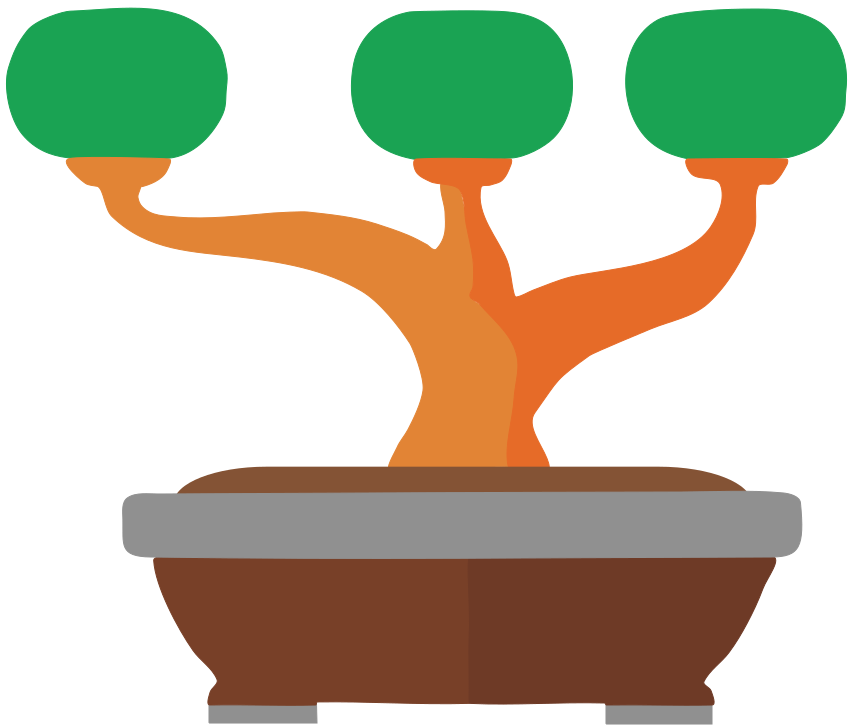
\includegraphics[width=4mm]{../figures/tidyparse_logo.png}} ([xshift=-10mm,yshift=-7mm]interior.north west);
    }
}

\newtcblisting{tidyoutput}[1][]{%
    width=8.5cm,
    left=10pt,
    top=1pt,
    listing options={
        basicstyle=\ttfamily\small,
%numberstyle=\footnotesize,
        showstringspaces=false,
        tabsize=2,
        breaklines=true,
        numbers=none,
        inputencoding=utf8,
        escapeinside={(*@}{@*)},
        #1
    }
}

\colorlet{lred}{red!30}
\colorlet{lorange}{orange!30}
\colorlet{lgreen}{green!30}
\colorlet{lgray}{black!15}
\DeclareRobustCommand{\hlred}[1]{{\sethlcolor{lred}\hl{#1}}}
\DeclareRobustCommand{\hlorange}[1]{{\sethlcolor{lorange}\hl{#1}}}
\DeclareRobustCommand{\hlgreen}[1]{{\sethlcolor{lgreen}\hl{#1}}}
\DeclareRobustCommand{\hlgray}[1]{{\sethlcolor{lgray}\hl{#1}}}

\usepackage{url}
\usepackage{qtree}

\usepackage{filecontents}
\usepackage{pstricks-add}
\usepackage{emoji}
\usepackage{alltt}
\usepackage{nicematrix}
\usepackage{graphicx}
\usepackage{ulem}
\usepackage{upquote}
